
\documentclass[12pt, a4paper]{report}
\usepackage{graphicx}
\usepackage{amsmath}
\usepackage{float}


\title{\textbf{EE2703 : Applied Programming Lab}\\Assignment 3} % Title

\author{Harisankar K J \\ EE20B043} % Author name

\date{18 February 2022} % Date for the report

\begin{document}		
		
\maketitle % Insert the title, author and date
\section*{Abstract}
Reading data from files and parsing them\\
– Analysing the data to extract information\\
– Study the effect of noise on the fitting process\\
– Plotting graphs\\
\section*{Tasks}
\subsection{Q1:Generation of Data}
Data generated using the generate script given is stored into the 'fitting.dat' file. the data contains the output of a function(a variation of Besel Function) along with noise.
\subsection{Q2:Loading the data into a matrix}
The data values in 'fitting.dat' is extracted and stored in a matrix.\\Code:
\begin{verbatim}
yf = np.loadtxt("fitting.dat")
(N, k) = yf.shape
t = yf[:, 0]
\end{verbatim}

\subsection{Q3:Plot of the Data to be Fitted}
Matplotlib is used the plot the values.\\Code:
\begin{verbatim}
scl = logspace(-1, -3, 9)
figure(0)
for i in range(1, k):
    plot(t, yf[:, i], label=("sigma = " + str(round(scl[i-1], 4))))
xlabel(r'$t$', size=20)
ylabel(r'$f(t)+n$', size=20)
title(r'Plot of the data to be fitted').
\end{verbatim}

\subsection{Q4:Plotting Original Function with A=1.05 and b=-0.105}
The original function is defined and plotted.\\Code:
\begin{verbatim}
def g(tk=t, A=1.05, B=-0.105):
    return A*sp.jn(2, tk)+B*t
y = g()
plot(t, y, label='true')
legend()
grid(True)
show()
\end{verbatim}
	\centering
	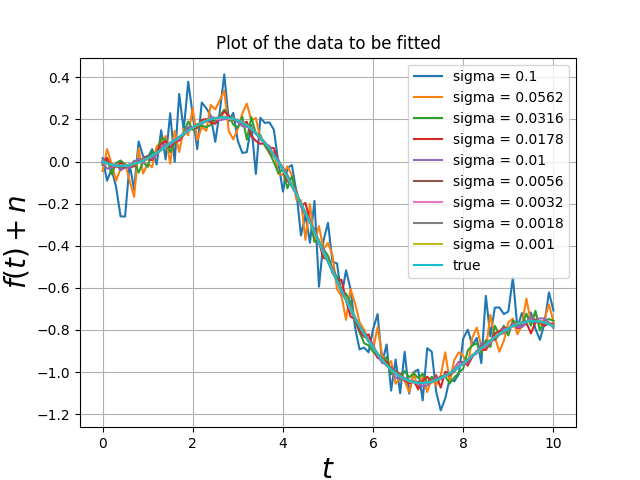
\includegraphics[scale=0.8]{Figure_0.png}
	\caption{Plot of All the Data Values along with true value.}
	
\subsection{Q5:Plotting Error-bars}
\begin{verbatim}
figure(1)
plot(t, y, label='true')
errorbar(t[::5], yf[:, 1][::5], scl[0], fmt='ro')
xlabel('$t\\rightarrow$')
title('Data Points with Error for St.Dev=0.10')
grid(True)
show()
\end{verbatim}
	\centering
	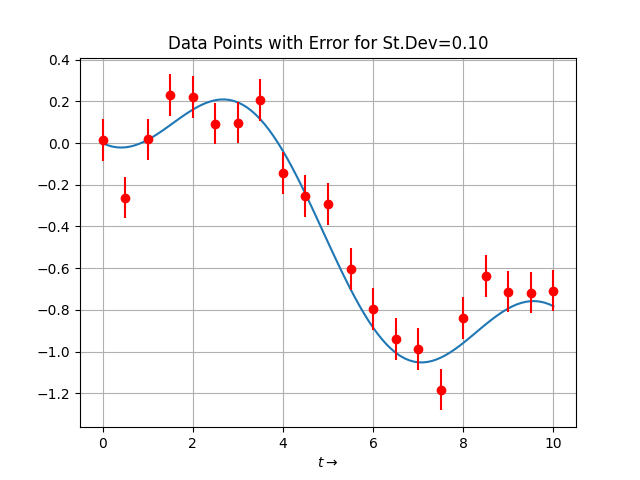
\includegraphics[scale=0.8]{Figure_1.png}  
	\caption{Error-bar Plotting}

\subsection{Q6:Comparing Data values of Generated Matrix and True Function Data Matrix}
Data value matrix generated and the true function data value matrix compared.
\begin{verbatim}
y1 = sp.jn(2, t)
M = c_[y1, t]
AB = array((1.05, -0.105))
if allclose(g(), dot(M, AB)):
    print("The values of the matrices match")
else:
    print("matrix values no  similar")
\end{verbatim}

\subsection{Q7:Generating Errors for different 'A' and 'B' and Finding Mean Square Error}
\begin{verbatim}
n = 21
A = linspace(0, 2, n)
B = linspace(-0.2, 0, n)
eps = np.zeros((n, n))
for i in range(n):
    for j in range(n):
        eps[i][j] = mean(square(yf[:, 1]-g(t, A[i], B[j])))
\end{verbatim}

\subsection{Q8:Plotting Contours of Mean Square Error}
\begin{verbatim}
figure(2)
pl = contour(A, B, eps, levels=20)
xlabel('$A\\rightarrow$')
ylabel('$B\\rightarrow$')
title(r'Contour Plot')
clabel(pl)
grid(True)
show()
\end{verbatim}
	\centering
	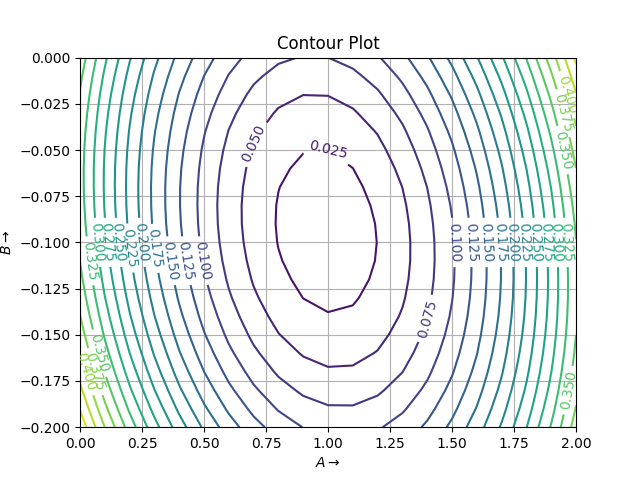
\includegraphics[scale=0.65]{Figure_2.png}  \\ 
	\caption{MS Error Contour}

\subsection{Q9:Estimating A and B}
The value of A and B as a matrix AB is estimated by using the data matrix from Q7.\\
Code:
\begin{verbatim}
ex = np.zeros((2, 1))
ex = scipy.linalg.lstsq(M, y)[0]
\end{verbatim}

\subsection{Q10:Error of A and B in Linear Scale}
The error in estimate is found out in linear scale and its variation with noise standard deviation is plotted.\\
Code:
\begin{verbatim}
fit = np.zeros((k-1, 2))
for i in range(k-1):
    fit[i] = scipy.linalg.lstsq(M, yf[:, i+1])[0]
Ae = np.zeros((k-1, 1))
Be = np.zeros((k-1, 1))
for i in range(k-1):
    Ae[i] = square(fit[i][0]-ex[0])
    Be[i] = square(fit[i][1]-ex[1])
figure(3)
plot(scl, Ae, label='A')
plot(scl, Be, label='B')
xlabel('Noise standard deviation')
ylabel('MS error')
title('Error in Estimate')
legend()
grid(True)
show()
\end{verbatim}
	\centering
	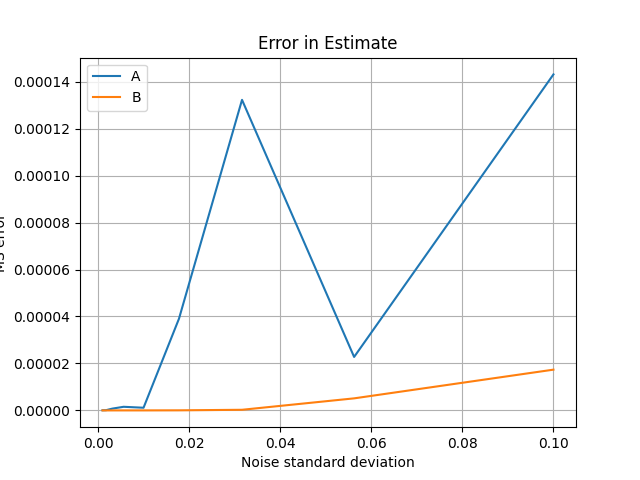
\includegraphics[scale=0.8]{Figure_3.png}
	\caption{Error on linear scale.}

\subsection{Q11:Error of 'A' and 'B' on log-log Scale}
Re-plotting the error in A and B in log-log scale.\\
code:
\begin{verbatim}
figure(4)
loglog(scl, Ae[:, 0], 'ro', label='A error(in logscale)')
loglog(scl, Be[:, 0], 'go', label='B error(in logscale)')
errorbar(scl, Ae[:, 0], std(Ae[:, 0]), fmt='ro')
errorbar(scl, Be[:, 0], std(Be[:, 0]), fmt='go')
xlabel('Noise Standard Deviation')
ylabel('MS Error (in logscale)')
title('Error in Estimate (in logscale)')
legend()
grid(True)
show()
\end{verbatim}
	\centering
	\includegraphics[scale=0.18]{Figure_4.png}
	\caption{Error on log-log Scale.}

\section*{Conclusion}
We used SciPy to analyse and estimate the coefficients of a function with noise values in the generated output of the function. We also understood that as noise vales in the data increases, the value of error in estimation of coefficients increases.

\end{document}



 